\begin{figure}[h!]
	\centering
	
	
	
	\tikzset{every picture/.style={line width=0.75pt}} %set default line width to 0.75pt        
	
	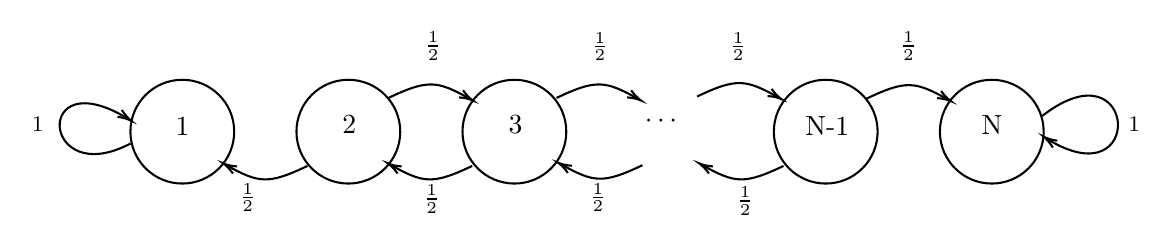
\begin{tikzpicture}[x=0.75pt,y=0.75pt,yscale=-1,xscale=1]
		%uncomment if require: \path (0,300); %set diagram left start at 0, and has height of 300
		
		%Shape: Circle [id:dp09774088338298847] 
		\draw   (100,125) .. controls (100,111.19) and (111.19,100) .. (125,100) .. controls (138.81,100) and (150,111.19) .. (150,125) .. controls (150,138.81) and (138.81,150) .. (125,150) .. controls (111.19,150) and (100,138.81) .. (100,125) -- cycle ;
		%Shape: Circle [id:dp43482816564378113] 
		\draw   (180,125) .. controls (180,111.19) and (191.19,100) .. (205,100) .. controls (218.81,100) and (230,111.19) .. (230,125) .. controls (230,138.81) and (218.81,150) .. (205,150) .. controls (191.19,150) and (180,138.81) .. (180,125) -- cycle ;
		%Shape: Circle [id:dp7628960050576648] 
		\draw   (260,125) .. controls (260,111.19) and (271.19,100) .. (285,100) .. controls (298.81,100) and (310,111.19) .. (310,125) .. controls (310,138.81) and (298.81,150) .. (285,150) .. controls (271.19,150) and (260,138.81) .. (260,125) -- cycle ;
		%Shape: Circle [id:dp3849023603262607] 
		\draw   (410,125) .. controls (410,111.19) and (421.19,100) .. (435,100) .. controls (448.81,100) and (460,111.19) .. (460,125) .. controls (460,138.81) and (448.81,150) .. (435,150) .. controls (421.19,150) and (410,138.81) .. (410,125) -- cycle ;
		%Shape: Circle [id:dp902561209940324] 
		\draw   (490,125) .. controls (490,111.19) and (501.19,100) .. (515,100) .. controls (528.81,100) and (540,111.19) .. (540,125) .. controls (540,138.81) and (528.81,150) .. (515,150) .. controls (501.19,150) and (490,138.81) .. (490,125) -- cycle ;
		%Curve Lines [id:da2277389625716164] 
		\draw    (224.33,108.74) .. controls (243.31,99.74) and (247.7,100.35) .. (263.26,109.02) ;
		\draw [shift={(265,110)}, rotate = 209.42] [color={rgb, 255:red, 0; green, 0; blue, 0 }  ][line width=0.75]    (6.56,-1.97) .. controls (4.17,-0.84) and (1.99,-0.18) .. (0,0) .. controls (1.99,0.18) and (4.17,0.84) .. (6.56,1.97)   ;
		%Curve Lines [id:da8597065575180056] 
		\draw    (305.33,108.74) .. controls (324.31,99.74) and (328.7,100.35) .. (344.26,109.02) ;
		\draw [shift={(346,110)}, rotate = 209.42] [color={rgb, 255:red, 0; green, 0; blue, 0 }  ][line width=0.75]    (6.56,-1.97) .. controls (4.17,-0.84) and (1.99,-0.18) .. (0,0) .. controls (1.99,0.18) and (4.17,0.84) .. (6.56,1.97)   ;
		%Curve Lines [id:da07306821532750352] 
		\draw    (454.67,109.08) .. controls (473.65,100.07) and (478.03,100.69) .. (493.59,109.36) ;
		\draw [shift={(495.33,110.33)}, rotate = 209.42] [color={rgb, 255:red, 0; green, 0; blue, 0 }  ][line width=0.75]    (6.56,-1.97) .. controls (4.17,-0.84) and (1.99,-0.18) .. (0,0) .. controls (1.99,0.18) and (4.17,0.84) .. (6.56,1.97)   ;
		%Shape: Boxed Bezier Curve [id:dp2584084656510479] 
		\draw    (185.33,141.51) .. controls (166.35,150.51) and (161.97,149.9) .. (146.41,141.23) ;
		\draw [shift={(144.67,140.25)}, rotate = 29.42] [color={rgb, 255:red, 0; green, 0; blue, 0 }  ][line width=0.75]    (6.56,-1.97) .. controls (4.17,-0.84) and (1.99,-0.18) .. (0,0) .. controls (1.99,0.18) and (4.17,0.84) .. (6.56,1.97)   ;
		%Shape: Boxed Bezier Curve [id:dp08231579755337615] 
		\draw    (264.67,141.51) .. controls (245.69,150.51) and (241.3,149.9) .. (225.74,141.23) ;
		\draw [shift={(224,140.25)}, rotate = 29.42] [color={rgb, 255:red, 0; green, 0; blue, 0 }  ][line width=0.75]    (6.56,-1.97) .. controls (4.17,-0.84) and (1.99,-0.18) .. (0,0) .. controls (1.99,0.18) and (4.17,0.84) .. (6.56,1.97)   ;
		%Shape: Boxed Bezier Curve [id:dp9912054198682547] 
		\draw    (346.67,141.17) .. controls (327.69,150.18) and (323.3,149.56) .. (307.74,140.89) ;
		\draw [shift={(306,139.92)}, rotate = 29.42] [color={rgb, 255:red, 0; green, 0; blue, 0 }  ][line width=0.75]    (6.56,-1.97) .. controls (4.17,-0.84) and (1.99,-0.18) .. (0,0) .. controls (1.99,0.18) and (4.17,0.84) .. (6.56,1.97)   ;
		%Shape: Boxed Bezier Curve [id:dp49752798194307046] 
		\draw    (414.67,141.51) .. controls (395.69,150.51) and (391.3,149.9) .. (375.74,141.23) ;
		\draw [shift={(374,140.25)}, rotate = 29.42] [color={rgb, 255:red, 0; green, 0; blue, 0 }  ][line width=0.75]    (6.56,-1.97) .. controls (4.17,-0.84) and (1.99,-0.18) .. (0,0) .. controls (1.99,0.18) and (4.17,0.84) .. (6.56,1.97)   ;
		%Curve Lines [id:da6769266285825299] 
		\draw    (373,108.08) .. controls (391.98,99.07) and (396.37,99.69) .. (411.93,108.36) ;
		\draw [shift={(413.67,109.33)}, rotate = 209.42] [color={rgb, 255:red, 0; green, 0; blue, 0 }  ][line width=0.75]    (6.56,-1.97) .. controls (4.17,-0.84) and (1.99,-0.18) .. (0,0) .. controls (1.99,0.18) and (4.17,0.84) .. (6.56,1.97)   ;
		%Curve Lines [id:da5266663507857827] 
		\draw    (539.33,117.41) .. controls (585.53,81.44) and (589.59,158.51) .. (541.47,128.36) ;
		\draw [shift={(540,127.41)}, rotate = 33.33] [color={rgb, 255:red, 0; green, 0; blue, 0 }  ][line width=0.75]    (6.56,-1.97) .. controls (4.17,-0.84) and (1.99,-0.18) .. (0,0) .. controls (1.99,0.18) and (4.17,0.84) .. (6.56,1.97)   ;
		%Curve Lines [id:da13630212552736864] 
		\draw    (100,130.74) .. controls (56.77,153.51) and (52.74,90.36) .. (98.92,118.85) ;
		\draw [shift={(100.33,119.74)}, rotate = 212.76] [color={rgb, 255:red, 0; green, 0; blue, 0 }  ][line width=0.75]    (6.56,-1.97) .. controls (4.17,-0.84) and (1.99,-0.18) .. (0,0) .. controls (1.99,0.18) and (4.17,0.84) .. (6.56,1.97)   ;
		
		% Text Node
		\draw (120.33,116.67) node [anchor=north west][inner sep=0.75pt]   [align=left] {1};
		% Text Node
		\draw (200.67,115.67) node [anchor=north west][inner sep=0.75pt]   [align=left] {2};
		% Text Node
		\draw (280.67,116) node [anchor=north west][inner sep=0.75pt]   [align=left] {3};
		% Text Node
		\draw (423.67,116.33) node [anchor=north west][inner sep=0.75pt]   [align=left] {N-1};
		% Text Node
		\draw (508.67,115.67) node [anchor=north west][inner sep=0.75pt]   [align=left] {N};
		% Text Node
		\draw (151,148.4) node [anchor=north west][inner sep=0.75pt]  [font=\footnotesize]  {$\frac{1}{2}$};
		% Text Node
		\draw (239.67,149.07) node [anchor=north west][inner sep=0.75pt]  [font=\footnotesize]  {$\frac{1}{2}$};
		% Text Node
		\draw (319.67,148.4) node [anchor=north west][inner sep=0.75pt]  [font=\footnotesize]  {$\frac{1}{2}$};
		% Text Node
		\draw (390.67,150.07) node [anchor=north west][inner sep=0.75pt]  [font=\footnotesize]  {$\frac{1}{2}$};
		% Text Node
		\draw (469.33,75.4) node [anchor=north west][inner sep=0.75pt]  [font=\footnotesize]  {$\frac{1}{2}$};
		% Text Node
		\draw (387.33,75.73) node [anchor=north west][inner sep=0.75pt]  [font=\footnotesize]  {$\frac{1}{2}$};
		% Text Node
		\draw (320.67,75.73) node [anchor=north west][inner sep=0.75pt]  [font=\footnotesize]  {$\frac{1}{2}$};
		% Text Node
		\draw (240.33,75.4) node [anchor=north west][inner sep=0.75pt]  [font=\footnotesize]  {$\frac{1}{2}$};
		% Text Node
		\draw (579.33,116.73) node [anchor=north west][inner sep=0.75pt]  [font=\footnotesize]  {$1$};
		% Text Node
		\draw (51,116.4) node [anchor=north west][inner sep=0.75pt]  [font=\footnotesize]  {$1$};
		% Text Node
		\draw (346.33,115.73) node [anchor=north west][inner sep=0.75pt]    {$\cdots $};
		
		
	\end{tikzpicture}
\end{figure}